%#BIBTEX pbibtex paper
% 以下の3行は変更しないこと.
\documentclass[T,dvipdfmx]{compsoft}
\taikai{2020}
\pagestyle {empty}

\usepackage [dvipdfmx] {graphicx}

% ユーザが定義したマクロなどはここに置く.ただし学会誌のスタイルの
% 再定義は原則として避けること.
\usepackage{multicol}
\usepackage{url}
%\usepackage{comments} % added by Banbara on 10th August
\newcommand{\bhline}{\noalign{\hrule height 1.5pt}}
%\renewcommand{\labelenumi}{(\arabic{enumi})}

%%% For ASP
\newcommand{\asap}{\textit{teaspoon}}
\newcommand{\gringo}{\textit{gringo}}
\newcommand{\clingo}{\textit{clingo}}
\newcommand{\clasp}{\textit{clasp}}
\newcommand{\dlv}{\textit{DLV}}
\newcommand{\wasp}{\textit{WASP}}
\newcommand{\code}[1]{\lstinline[basicstyle=\ttfamily]{#1}}
\newcommand{\naf}[1]{\ensuremath{{\sim\!\!{#1}}}}
\newcommand{\head}[1]{\ensuremath{\mathit{head}(#1)}}
\newcommand{\body}[1]{\ensuremath{\mathit{body}(#1)}}
%\newcommand{\atom}[1]{\ensuremath{\mathit{atom}(#1)}}
\newcommand{\poslits}[1]{\ensuremath{{#1}^+}}
\newcommand{\neglits}[1]{\ensuremath{{#1}^-}}
\newcommand{\pbody}[1]{\poslits{\body{#1}}}
\newcommand{\nbody}[1]{\neglits{\body{#1}}}
%\newcommand{\Cn}[1]{\ensuremath{\mathit{Cn}(#1)}}
\newcommand{\reduct}[2]{\ensuremath{#1^{#2}}}


\usepackage{tikz}
\usetikzlibrary{arrows,shapes,calc,intersections}
\usetikzlibrary{positioning}
\usetikzlibrary{fit}

%\newcommand{\nodeVP}[3]{
  \coordinate[#2] (#1);
  \draw[fill=cyan!30] (#1)--+(-1,0)--+(0,1)--+(1,0)--cycle;
  \draw (#1)node[above]{\tiny{#3}};
  \draw[fill=black] (#1) +(-0.5,0.5)--+(0.5,0.5)--+(0,1)--cycle;
  \node[rectangle,above=0.5cm of #1,white](vp){\tiny{VP}};
  \coordinate[below=0.5cm of #1] (via_#1);
  \draw (via_#1)node[above right]{\tiny{[1..1]}};
  \draw (via_#1) +(170:0.2) arc (170:370:0.2);
  \draw (#1)--(via_#1);

}
\newcommand{\nodeTrans}[3]{
  \coordinate[#2] (#1);
  \draw[fill=cyan!30] (#1)--+(-1,0)--+(0,1)--+(1,0)--cycle;
  \draw (#1)node[above]{\tiny{#3}};
  \draw[fill=black] (#1) +(-0.5,0.5)--+(0.5,0.5)--+(0,1)--cycle;
  \node[rectangle,above=0.5cm of #1,white](vp){\tiny{VP}};
  \coordinate[below=1.7cm of #1] (via_#1);
  \draw (via_#1)node[below=0.2cm]{\tiny{[1..1]}};
  \draw (via_#1) +(135:0.2) arc (135:405:0.2);
  \draw (#1)--(via_#1);

}

\newcommand{\nodeVPdashed}[3]{
  \coordinate[#2] (#1);
  \draw[fill=cyan!30,dashed] (#1)--+(-1,0)--+(0,1)--+(1,0)--cycle;
  \draw (#1)node[above]{\tiny{#3}};
  \fill[black] (#1) +(-0.5,0.5)--+(0.5,0.5)-- +(0,1)--cycle;
  \node[rectangle,above=0.5cm of #1,white](vp){\tiny{VP}};
  \coordinate[below=0.5cm of #1] (via_#1);
  \draw (via_#1)node[above right]{\tiny{[1..1]}};
  \draw (via_#1) +(-0.2,0) arc (180:360:0.2);
  \draw (#1)--(via_#1);

}

\newcommand{\nodeV}[4]{
  \node [draw,inner xsep=2pt,#2,fill=black!10,font=\tiny] (#1){
      \begin{tabular}{l}
       #3\\
       #4\\
      \end{tabular}
  };
  \fill [black] (#1.north west)--++(0,-2mm)--++(1mm,0)--++(1mm,0)--++(0,2mm); 
  \draw (#1.north west) ++(1mm,-1mm) node[white]{\tiny{v}};
}

\newcommand{\nodeVchoiced}[4]{
  \node [draw,inner xsep=2pt,#2,fill=red!50,font=\tiny] (#1){
      \begin{tabular}{l}
       #3\\
       #4\\
      \end{tabular}
  };
  \fill [black] (#1.north west)--++(0,-2mm)--++(1mm,0)--++(1mm,0)--++(0,2mm); 
  \draw (#1.north west) ++(1mm,-1mm) node[white]{\tiny{v}};

}


\usepackage{listings}
\usepackage{plistings}
\def\lstlistingname{コード}


% \lstset{
%  basicstyle=\ttfamily\tiny\color{black},
%  keepspaces=true,
%  columns=[l]{fullflexible},
%  escapechar=|,
%  commentstyle={\color{red}},
%  stringstyle={\color{blue}},
% }
% ユーザが定義したマクロなどはここに置く.ただし学会誌のスタイルの
% 再定義は原則として避けること

%%% figureテンプレ %%%%%%%%%%%%%%%%%%%%%%%%%%%%%%
% \begin{figure}[tb]
%  \centerline {\includegraphics {images/XX.eps}}
%  \caption{}
%  \label{fig:}
% \end{figure}
%%%%%%%%%%%%%%%%%%%%%%%%%%%%%%%%%%%%%%%%%%%%%%%%

\begin{document}

% 論文のタイトル
\title{車両装備仕様問題に対する解集合プログラミングの適用}

% 著者
% 和文論文の場合,姓と名の間には半角スペースを入れ,
% 複数の著者の間は全角スペースで区切る
%
\author{竹内 頼人 田村 直之 番原 睦則
%
% ここにタイトル英訳 (英文の場合は和訳) を書く.
%
\ejtitle{Applying Answer Set Programming to Vehicle Equipment Specification Problem}
%
% ここに著者英文表記 (英文の場合は和文表記) および
% 所属 (和文および英文) を書く.
% 複数著者の所属はまとめてよい.
%
\shozoku{Raito Takeuchi, Mutsunori Banbara}{名古屋大学 大学院情報学研究科}%
{Graduate School of Informatics, Nagoya University}
\shozoku{Naoyuki Tamura}{神戸大学 情報基盤センター}%
{Information Science and Technology Center, Kobe University}}


% 和文アブストラクト
\Jabstract{%
  車両装備仕様とは,簡単に言うと,自動車のカタログに記載されているモデ
  ル/グレードと装備の組合せのことである.車両装備仕様問題は,与えられ
  た装備仕様の個数,装備タイプの集合,装備オプションの集合などから,装
  備および燃費に関する制約を満たしつつ,予想販売台数を最大化する車両装
  備仕様を求める問題である.
  % 
  本論文では,企業平均燃費(Corporate Average Fuel Efficiency; CAFE)方式
  と呼ばれる燃費規制に基づく車両装備仕様問題に対して,
  解集合プログラミング(Answer Set Programming; ASP)を用いたソルバーの実
  装と評価について述べる.
  提案手法は,まず与えられた問題インスタンスを ASP のファクト形式に変
  換した後,それらファクトと車両装備仕様問題を解くための ASP 符号化と
  結合した上で,高速ASPシステムを用いて解を求める.
  % 
  ASP符号化として,基本符号化と改良符号化の2種類を考案した.
  特に,改良符号化は,装備仕様の燃費や予想販売台数を算出するために必要
  な ASP のルール数を少なく抑えるよう工夫されており,大規模な問題への
  有効性が期待できる.
  また,製造ラインの削減や大量生産を促進することを狙いとして,予想販売
  台数の最大化に加えて,装備オプション数の最小化も行える拡張符号化につ
  いても触れる.
  % 
  最後に,提案手法の評価として,企業から提供を受けた実用規模の問題イン
  スタンスを含む問題集を用いた実験結果について述べる.
}

\maketitle \thispagestyle {empty}


% ここから「本文」
\section{はじめに}\label{sec:introduction}
% ------------------------------------------
  \thicklines
  \setlength{\unitlength}{1.28pt}
  \small
  \begin{picture}(280,57)(4,-10)
    \put(  0, 20){\dashbox(50,24){\shortstack{根付き全域森\\問題}}}
    \put( 60, 20){\framebox(50,24){変換器}}
    \put(120, 20){\dashbox(50,24){\shortstack{ASPファクト}}}
    \put(120,-10){\alert{\bf\dashbox(50,24){\scriptsize{\shortstack{ASP符号化\\(論理プログラム)}}}}}
    \put(180, 20){\framebox(50,24){ASPシステム}}
    \put(240, 20){\dashbox(50,24){\shortstack{根付き全域森\\問題の解}}}
    \put( 50, 32){\vector(1,0){10}}
    \put(110, 32){\vector(1,0){10}}
    \put(170, 32){\vector(1,0){10}}
    \put(230, 32){\vector(1,0){10}}
    \put(170, +2){\line(1,0){4}}
    \put(174, +2){\line(0,1){30}}
  \end{picture}  

% ------------------------------------------

車両装備仕様とは,簡単に言うと,自動車のカタログに記載されているモデ
ル/グレードと装備の組合せのことである.
車両装備仕様を決めるには,販売される国や地域の法規や規制,
地域や市場の特性,市場の嗜好や競合など十分に考慮する必要があり,
現状では専門知識をもつ技術者の多大な労力が費やされている.
そのため,車両装備仕様探索の自動化・効率化は自動車メーカーにとって
重要な課題の一つである.

\textbf{多目的車両装備仕様問題}は組合せ最適化問題の一種であり,主に装備タイ
プと装備オプションから構成される.
\textbf{装備タイプ}はエンジンやトランスミッションなどの装備の種類を表す.
\textbf{装備オプション}は4気筒エンジン,CVTなどの具体的な装備を表す.
多目的車両装備仕様問題の目的は,
与えられた装備仕様の個数,
装備タイプの集合,
装備オプションの集合から,
装備および燃費に関する制約を満たしつつ,
予想販売台数の最大化や装備オプション数の最小化など,トレードオフの関係にある
複数の目的関数のもとで最適な車両装備仕様を求めることである.

本研究では,燃費に関する制約として,欧米で採用され日本でも2020年度から
導入されている\textbf{企業平均燃費}
(Corporate Average Fuel Efficiency; CAFE~\cite{metimlit18:cafe})
方式を用いる.
このCAFE方式は自動車の燃費規制で,車種別ではなくメーカー全体での出荷台
数を加味した平均燃費を算出し,規制をかける方式である.
CAFE方式の特長は,ある特定の車種では燃費基準を達成できなくても,他の車
種の燃費を向上させることで基準を達成できることが可能な点である.
本論文では,CAFE方式に基づく多目的車両装備仕様問題(以降,\textbf{多目的CAFE問題}と
呼ぶ)を対象とする.

\textbf{解集合プログラミング}
(Answer Set Programming; ASP~\cite{%
  Baral03:cambridge,%
  Gelfond88:iclp,%
  Inoue08:jssst})
は,論理プログラミングから派生した宣言的プログラミングパラダイムである.
ASP言語は一階論理に基づく知識表現言語の一種である.
論理プログラムはASPのルールの有限集合である.
ASPシステムは論理プログラムから安定モデル意味論~\cite{Gelfond88:iclp}
に基づく解集合を計算するシステムである.
近年,SATソルバー技術を応用した高速ASPシステムが実現され,
ロボット工学,システム生物学,システム検証,制約充足問題,プランニング
など様々な分野への実用的応用が急速に拡大している~\cite{Gelfond16:aim}.


提案手法の有効性を評価するために,企業から提供を受けた小規模・中規模・大規模の
多目的CAFE問題に対して実行実験を行った結果,
小規模な問題では5問中4問で最適解の全列挙をすることができた.
\section{CAFE問題}\label{sec:background}

%-------------------------------------------------------
\begin{figure*}[t]
  \centering
  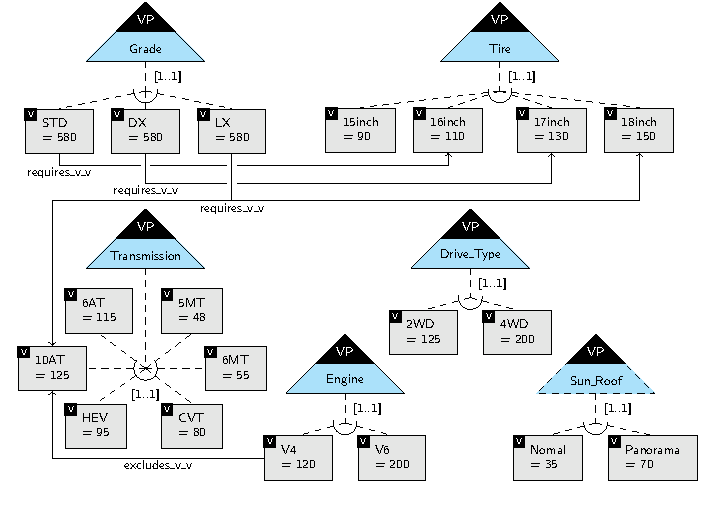
\includegraphics[width=0.8\linewidth]{images/ovm_example.pdf}
  \caption{CAFE問題の例}
  \label{fig:ovm_example}
\end{figure*}
%-------------------------------------------------------

CAFE問題の入力は以下の通りである.
以降,
装備タイプをタイプ,
装備オプションをオプション
と簡単に書くことにする.
\begin{enumerate}
\item タイプの集合\label{input:vp}
\item オプションの集合\label{input:v}
\item タイプとオプションの対応関係\label{input:vp-v}
\item 各タイプで選択可能なオプション数の上下限値\label{input:ublb}
\item タイプ同士,オプション同士,および,タイプとオプション間の依存関係
  \label{input:dependency}
\item 各オプションに付加された IWR 値\label{input:iwr}
%%%
\item 求めたい装備仕様の個数\label{input:g}
\item 各装備仕様とタイプ(あるいはオプション)間の依存関係\label{input:init}
\item 各装備仕様に含まれるオプションの IWR 値の総和と燃費との対応表\label{input:fe}
\item 各装備仕様に含まれるオプションの IWR 値の総和と予想販売台数との対応表\label{input:sv}
\item CAFE 基準値\label{input:cafe}
\end{enumerate}
入力~\ref{input:iwr}の IWR は Inertial Working Rating の略で,
直観的には各オプションの重量を表す.
入力~\ref{input:g}の個数は,求めたい派生車両の数と考えるとわかりやすい.
CAFE問題は,上記の入力から,
装備および燃費に関する制約を満たしつつ,
予想販売台数を最大化する車両装備仕様を求める問題である.

CAFE問題の制約は以下の通りである.
\begin{description}
\item[範囲制約]: 各装備仕様について,各タイプで選択されるオプション数は,
  入力~\ref{input:ublb}で与えられた上下限値の範囲内でなければならない.
\item[依存制約]: 各装備仕様について,入力~\ref{input:dependency}で与
  えられた依存関係を満たさなければならない.
  依存制約には,要求制約と排他制約の2つがある.
\item[燃費制約]: 入力~\ref{input:cafe}の CAFE 基準値を$t$,
  入力~\ref{input:g}の装備仕様個数を$n$として,
  以下の CAFE 規制を満たさなければならない.
  \begin{adjustvboxheight}
  \[
    \begin{array}{lcr}
      & & \\
      \displaystyle\frac{\sum_{i=1}^{n} FE_{i}\cdot SV_{i}}{\sum_{i=1}^{n} SV_{i}}
      &
        \geq 
      &
        t \\
      & & 
    \end{array}
  \]
  \end{adjustvboxheight}
  不等式の左辺は$n$個の装備仕様の\textbf{平均燃費}を表している.
  $FE_{i}$と$SV_{i}$は,装備仕様$i$の燃費と予想販売台数を表しており,
  それぞれ,入力~\ref{input:fe}と\ref{input:sv}の対応表を元に計算される.
\item[初期制約]:
  入力~\ref{input:init}で与えられた依存関係を満たさなければならない.
\end{description}

%%%%%%%%%%%%%%%%%%%%%%%%%%%%
%-------------------------------------------------------
\begin{figure}[tb]
  \centering
  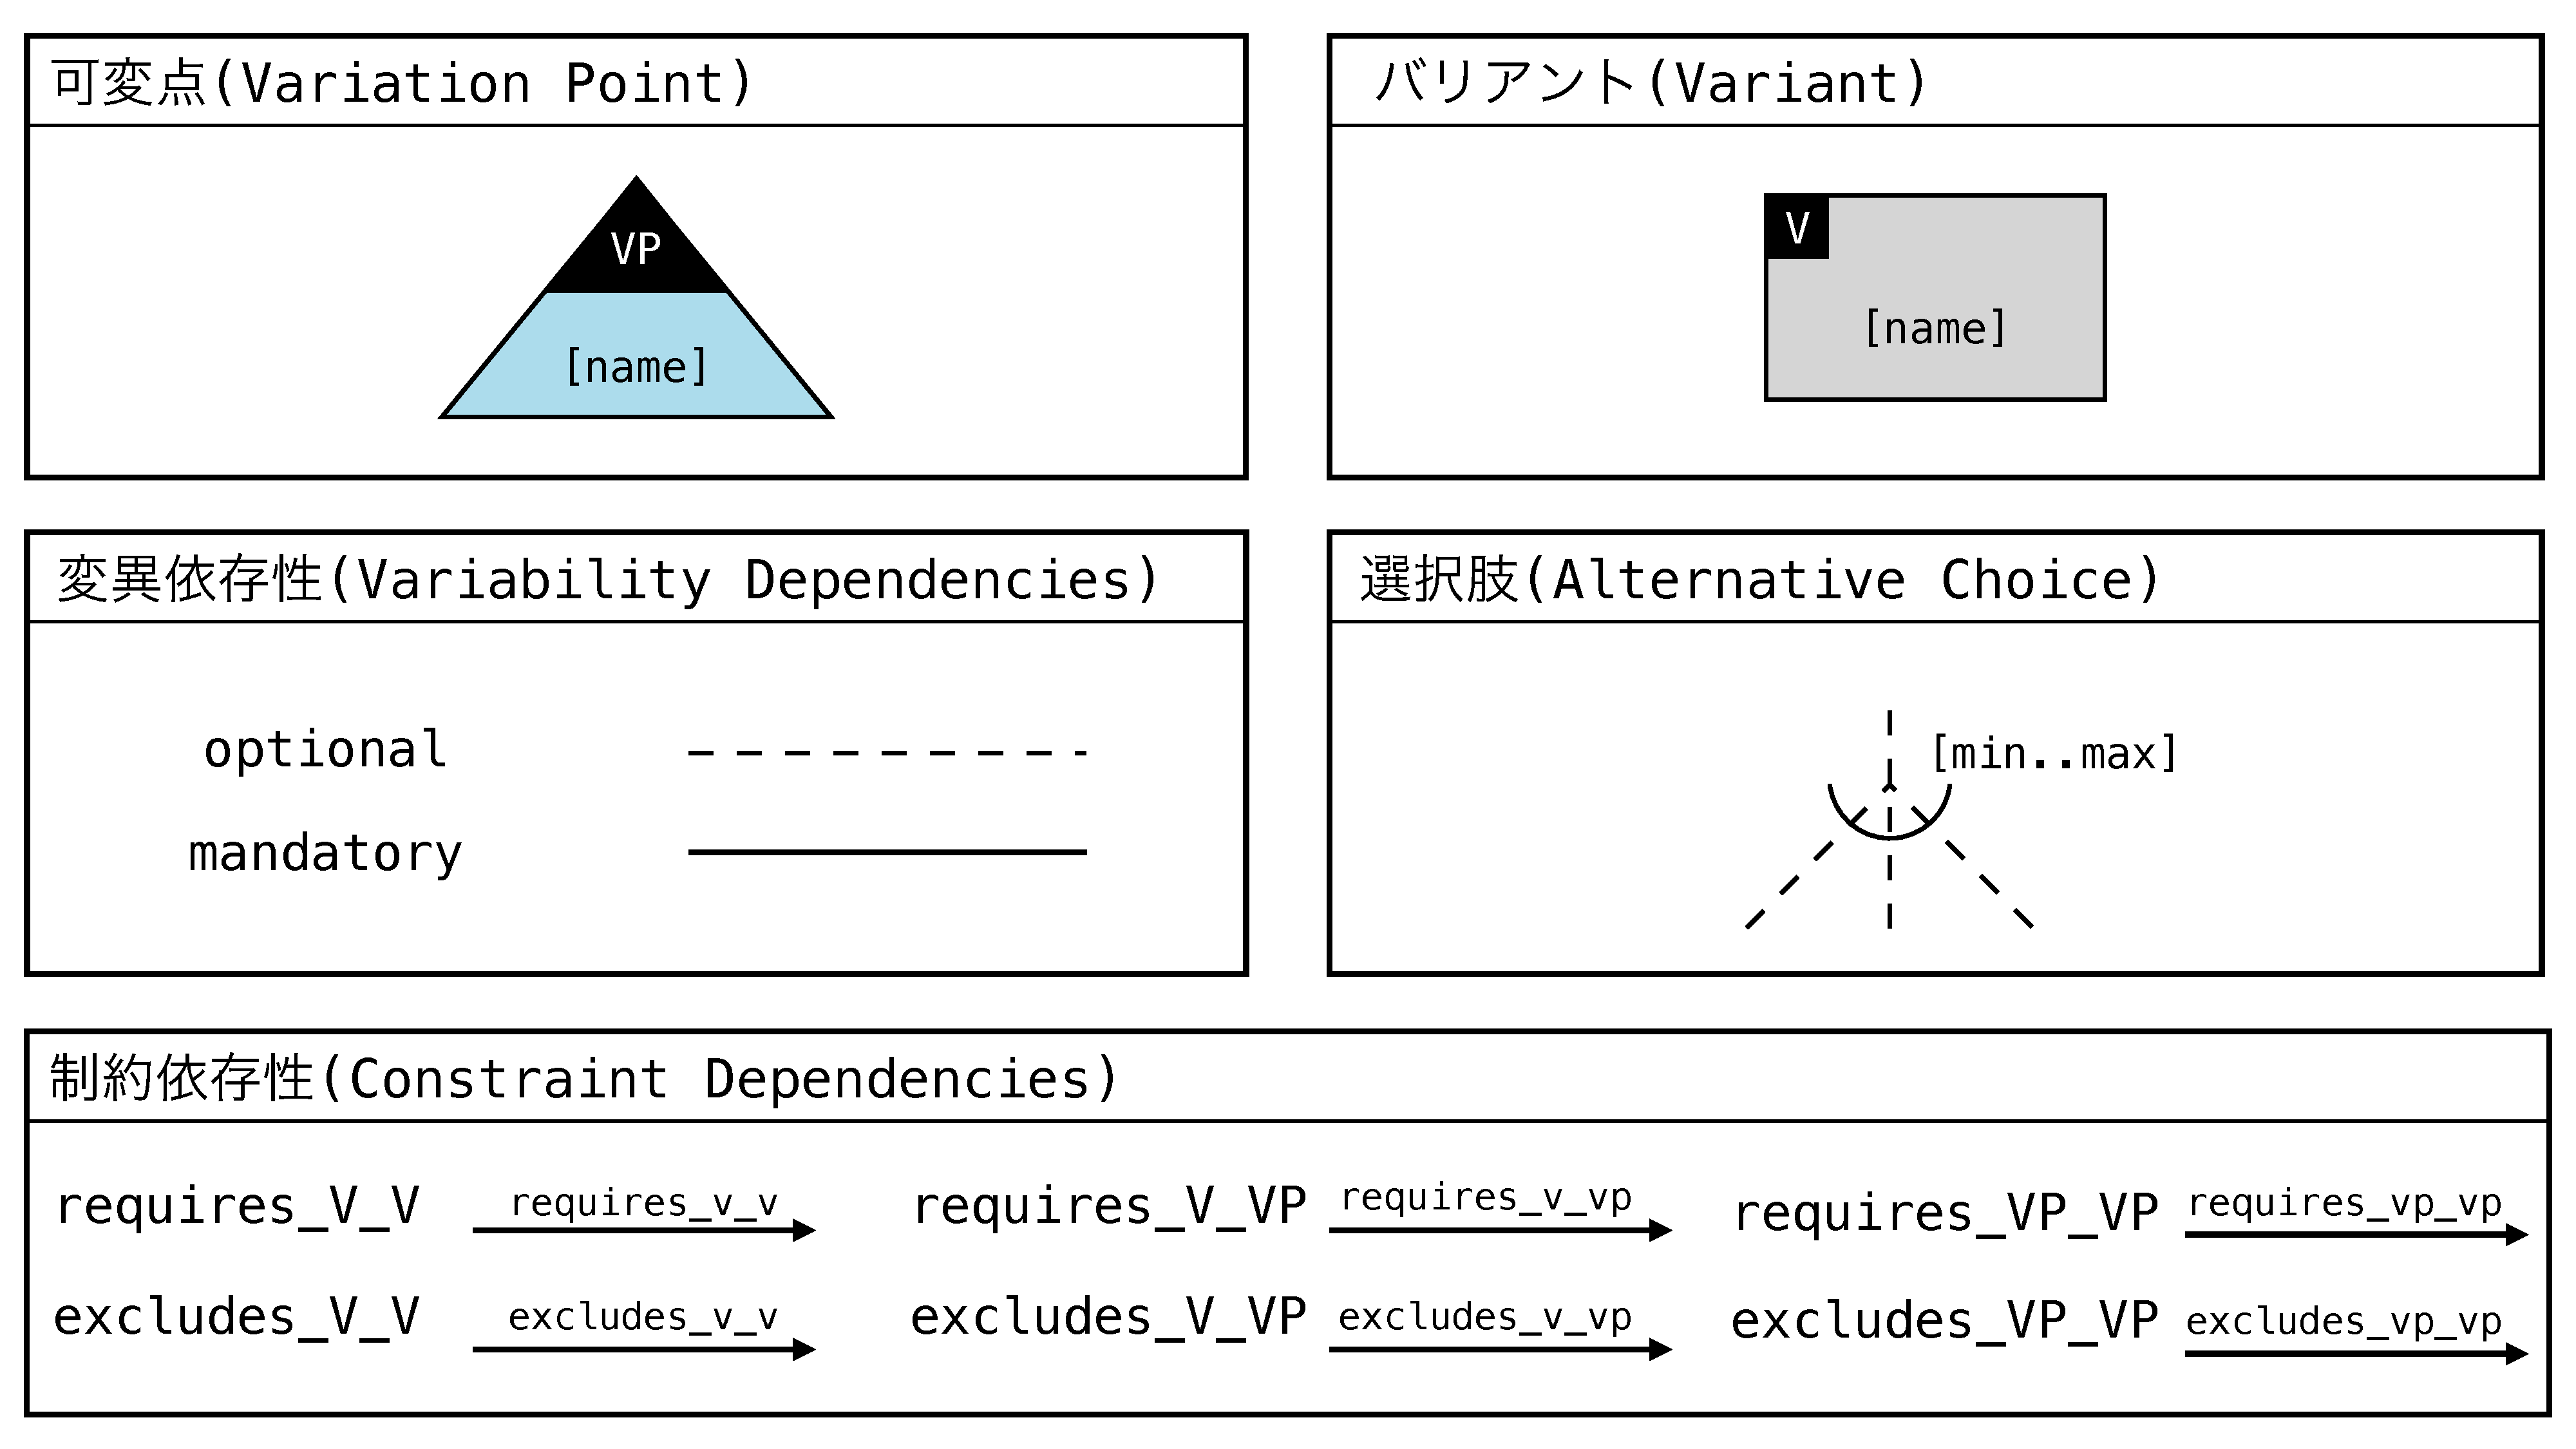
\includegraphics[width=\linewidth]{images/notation.pdf}
  \caption{可変性モデルの表記法\cite{Pohl05:sple}}
  \label{fig:ovm_notation}
\end{figure}
%-------------------------------------------------------

CAFE問題の例を図~\ref{fig:ovm_example}に示す.
この例は,ソフトウェアプロダクトライン開発の分野で用いられる
\textbf{可変性モデル} (Orthogonal Variability Model; OVM\cite{Pohl05:sple})
によって記述されている.
図~\ref{fig:ovm_notation}に,可変性モデルの基本的な表記法を示す.
可変性モデルでは,
仕様ごとに変わりうる項目を\textbf{可変点}と呼び,三角形で表す.
可変点の具体的なインスタンスを\textbf{バリアント}と呼び,長方形で表す.
可変点とバリアントの対応関係には\textbf{変異依存性}と\textbf{選択肢}があり,
選択肢の場合は,その多重度も付記される.
可変点同士,バリアント同士,および,可変点とバリアント間の依存関係は,
\textbf{制約依存性}によって表される.
制約依存性には,要求(\textsf{requires})と排除(\textsf{excludes})の2種類がある.

可変性モデルでCAFE問題を記述する場合,
タイプは可変点,
オプションとその IWR 値はバリアント,
タイプとオプションの対応関係および
選択可能なオプション数の上下限値は選択肢,
タイプ同士,オプション同士,および,タイプとオプション間の依存関係は
制約依存性によって表される.
以上から,CAFE問題の入力のうち,
\ref{input:vp}〜\ref{input:iwr}は可変性モデルによって記述されるこ
とがわかる.

図~\ref{fig:ovm_example}の問題例は,
6個のタイプ,19個のオプション,5個の依存制約から構成され,
各タイプの選択可能なオプション数はすべて1である.
本論文では,可変点で表されるタイプは,各装備仕様に対して必須とする.
ただし,\textsf{Sun\_Roof}のような選択可能なタイプ(必須ではないタイプ)
については,破線の可変点で表すものとする.

%-------------------------------------------------------
\begin{table}[t]
  \centering
  \caption{CAFE問題(図~\ref{fig:ovm_example})の解}
  \begin{tabular}{l|l|c|c|c} \bhline
    %\multicolumn{1}{c|}{装備}   & \multicolumn{3}{c}{装備仕様} \\ \cline{2-4}
    \multicolumn{2}{l|}{装備仕様}               & 1	& 2 	 & 3	\\  \hline
    装備 & \textsf{Grade}        & \textsf{STD}    & \textsf{DX}     & \textsf{LX}\\
    &\textsf{Drive\_Type}  & \textsf{2WD}    & \textsf{2WD}    & \textsf{2WD}\\
    &\textsf{Engine}	  & \textsf{V4}     & \textsf{V6}     & \textsf{V6}\\
    &\textsf{Tire}	  & \textsf{16inch} & \textsf{17inch} & \textsf{18inch}\\
    &\textsf{Transmission} & \textsf{5MT}    & \textsf{6MT}    & \textsf{10AT}\\
    &\textsf{Sun\_Roof}    & -               & \textsf{Normal} & -  \\ \hline
    \multicolumn{2}{l|}{IWR 値の総和}           & 983  & 1,125   & 1,180 \\ %\hline
    \multicolumn{2}{l|}{燃費(km/L)}      & 10.2  & 8.9     & 8.5 \\ %\hline
    \multicolumn{2}{l|}{予想販売台数}    & 745   & 1,988   & 1,171  \\ \hline
    \multicolumn{2}{l|}{平均燃費(km/L)}  & \multicolumn{3}{c}{9.0} \\ 
    \multicolumn{2}{l|}{予想販売台数(合計)}  & \multicolumn{3}{c}{3,904} \\ \hline
 \end{tabular}
 \label{tab:ovm_ans}
\end{table}
%-------------------------------------------------------

図~\ref{fig:ovm_example}の問題に対する解の例を表\ref{tab:ovm_ans}に示す.
この解は,
CAFE 基準値に9.0km/L,
求めたい装備仕様の個数に3を与え,
装備仕様とオプションの依存関係として,
(装備仕様1, \textsf{STD}),
(装備仕様2, \textsf{DX}),
(装備仕様3, \textsf{LX})
を要求して得られたものである.
各装備仕様の燃費(km/L)は,左から順に 10.2, 8.9, 8.5 と
個々には CAFE 基準値を満たしていないが,
3台の平均燃費は 9.028km/L となり,CAFE 規制を満たしている.


%%% Local Variables:
%%% mode: japanese-latex
%%% TeX-master: "paper"
%%% End:

\section{解集合プログラミング}\label{sec:asp}

ASPの言語は,
一般拡張選言プログラム
(General Extended Disjunctive Program)
をベースとしている\cite{Inoue08:jssst}.
本節では,説明の簡略化のため,そのサブクラスである
標準論理プログラムについて説明する.
以降,標準論理プログラムを単に論理プログラムと呼ぶ.

\textbf{論理プログラム}は,以下の形式の\textbf{ルール}の有限集合である.
\begin{equation}
  \label{eq:rule}
  a_0\leftarrow a_1,\dots,a_m,\naf{a_{m+1}},\dots,\naf{a_n}
\end{equation}
このルールの直観的な意味は,
「$a_1,\ldots,a_m$がすべて成り立ち,$a_{m+1},\ldots,a_n$のそれぞれが成
り立たないならば,$a_0$が成り立つ」である.
ここで,
$0\leq m\leq n$ であり,
各$a_i$はアトム,
$\naf{}$は\textbf{デフォルトの否定}
\footnote{\textbf{失敗による否定}とも呼ばれる.述語論理で定義される否定($\neg$)とは意味が異なる.},
``$,$''は連言を表す.
$\leftarrow$の左側を\textbf{ヘッド},右側を\textbf{ボディ}と呼ぶ.
ボディが空のルール(すなわち\(a_0\leftarrow\))を\textbf{ファクト}と呼び,
$\leftarrow$を省略してよい.

ヘッドが空のルールを\textbf{一貫性制約}と呼び,以下のように表す.
\begin{equation}
  \label{eq:constr}
  \leftarrow a_1,\dots,a_m,\naf{a_{m+1}},\dots,\naf{a_n}
\end{equation}
例えば,一貫性制約
``\(\leftarrow a_1,a_2\)''は,「$a_1$と$a_2$が両方同時に成り立つことはない」を意味し,
``\(\leftarrow a_1, \naf{a_{2}}\)''は,「$a_1$が成り立つならば,$a_2$が成り立つ」を意味する.

ASP言語には,組合せ問題を簡潔に記述するために,
\textbf{アグリゲート}(aggregate)と呼ばれる拡張構文がいくつか用意されている.
例えば,\textbf{選択子}``$\{a_1;\ldots;a_n\}$.''は,
アトム集合\(\{a_1,\ldots,a_n\}\)の任意の部分集合を解集合に含めることを意味する.
\textbf{個数制約}は選択子の両端に選択可能な個数の上下限を付けたものである.
例えば,``\(lb\ \{a_1;\dots;a_n\}\ ub \leftarrow Body\)''と書くと,
「$Body$が成り立つならば,$a_1,\dots,a_n$のうち,$lb$個以上$ub$個以下
が成り立つ」を意味する.
\textbf{重み付き個数制約}``\(t = \#sum\ \{w_1:a_1;\ldots;w_n:a_n\}\).''は,
$a_1,\dots,a_n$のうち真となるアトムの重み和が項$t$に等しくなることを意味する.
項$w_i$は重みを表し,演算子としては``=''以外にも``$\leq$'',``$\geq$''などを使用できる.
さらに,重み付き個数制約の``$\#sum$''を,``$\#max$''や``$\#min$''に書
き換えると,重み和ではなく,真となるアトムの重みの最大値や最小値を求め
ることができる.また,組合せ最適化問題を解くために,最小化関数
(\code{#minimize})・最大化関数(\code{#maximize})等も用意されている.

近年,
{\clingo}~\footnote{\url{https://potassco.org/}},
{\dlv}~\footnote{\url{http://www.dlvsystem.com/dlv/}},
{\wasp}~\footnote{\url{https://www.mat.unical.it/ricca/wasp/}}
など,SATソルバー技術を応用した高速なASPシステムが開発されている.
なかでも{\clingo}は,高性能かつ高機能なASPシステムとして世界中で広く使われている.
これらの高速ASPシステムは,変数を含む論理プログラムを変数を含まない論
理プログラムに変換(\textbf{基礎化})したのち,ASPソルバーを用いて解集合を計算する.
本論文で使用するASPシステム{\clingo}は,基礎化のためのグラウンダー
{\gringo}とASPソルバー{\clasp}をシームレスに結合したものである.

\begin{table}[tb]
  \centering
  \caption{論理プログラムとソースコードの対応}
  \tabcolsep = 2mm
  \begin{tabular}{l|*{6}{c}}\small
    論理プログラム &  $\leftarrow$ & $,$      & $;$      & $\sim$    & $\#sum$   \\\hline
    ソースコード   &  \code{:-}    & \code{,} & \code{;} & \code{not}& \code{#sum}
  \end{tabular}
  \label{tbl:map}
\end{table}

以降の節で示す論理プログラムのソースコードはすべて{\gringo}言語で書か
れており,表記上の対応については表~\ref{tbl:map}の通りである.

%%% Local Variables:
%%% mode: japanese-latex
%%% TeX-master: "paper"
%%% End:

\section{ASPに基づくCAFE問題ソルバー}

提案するCAFE問題ソルバーは,与えられた問題インスタンスをASPの
ファクト形式に変換した後,それらファクトとCAFE問題を解くためのASP符号
化(論理プログラム)を結合した上で,高速ASPシステム{\clingo}を用いて解
を求める(図~\ref{fig:arch}参照).
本節では,CAFE問題の入力と制約を論理プログラムとして表現する方法に
ついて述べる.
本論文では,説明の簡単化のため,
各タイプが選択可能なオプション数の上下限値を1とする.


%%%%%%%%%%%%%%%%%%%%%%%%%%%%%%%%%%%%
\subsection{ASPファクト形式}

%----------------------------------------
\lstinputlisting[float=htbp,caption={%
  CAFE問題の例(図~\ref{fig:ovm_example})のファクト表現.
  装備仕様の個数:3,
  装備仕様とオプションの依存関係:
  (装備仕様1, \textsf{STD}),
  (装備仕様2, \textsf{DX}),
  (装備仕様3, \textsf{LX})},%
captionpos=b,frame=single,label=code:ovm.lp,%
numbers=none,%
breaklines=true,%
columns=fullflexible,keepspaces=true,%
xrightmargin=1zw,% 
xleftmargin=1zw,% 
basicstyle=\ttfamily\scriptsize]{codes/ovm.lp} 
%----------------------------------------

CAFE 問題の入力は,CAFE 基準値(入力~\ref{input:cafe})
を除いて,ASP のファクトで表される.
CAFE 基準値は ASP の定数\code{t}で表すものとし,
実行時に{\clingo}のオプションから値を指定する.

CAFE 問題の例(図~\ref{fig:ovm_example})
をファクトで表現したものをコード~\ref{code:ovm.lp}に示す.
この2つを見比べると,可変性モデルの
可変点,
バリアント,
制約依存性(要求),
制約依存性(排除)が,
それぞれファクト
\code{vp_def/1}, 
\code{v_def/3},
\code{require_v_v/2},
\code{exclude_v_v/2}
に対応していることがわかる.
例えば,バリアント\textsf{V4}は,ファクト
\code{v_def("V4", "Engine", 120).}に対応している.
%
可変性モデルは CAFE 問題の入力~\ref{input:vp}〜\ref{input:iwr}を含んでいる.
%
この他,
\code{require_vp/1}は必須タイプ,
\code{group/1}は装備仕様の識別子(入力~\ref{input:g}),
\code{require_g_v/2}は
各装備仕様とオプション間の依存関係を表している(入力~\ref{input:init}).
例えば,\code{require_g_v(1, "STD").}は,装備仕様~\code{1}が
オプション\code{STD}を要求することを表す.

IWR 値の総和と燃費の対応表(入力~\ref{input:fe})は,
ファクト\texttt{fe\_map($S$,$FE$)}の有限集合で表される.
ここで,$S$はIWR 値の総和,$FE$は燃費を表す.
同様にして,
IWR 値の総和と予想販売台数の対応表(入力~\ref{input:sv})は,
ファクト\texttt{sv\_map($S$,$SV$)}の有限集合で表される.

%%%%%%%%%%%%%%%%%%%%%%%%%%%%%%%%%%%%
\subsection{CAFE問題の ASP 符号化}

%----------------------------------------
\lstinputlisting[float=tb,caption={%
  基本符号化},%
captionpos=b,frame=single,label=code:basic1.lp,%
numbers=left,%
breaklines=true,%
columns=fullflexible,keepspaces=true,%
xrightmargin=1zw,% 
xleftmargin=1zw,% 
basicstyle=\ttfamily\scriptsize]{codes/basic1.lp} 
%----------------------------------------

CAFE問題の各制約は,ASP の個数制約および一貫性制約を使って簡潔に表現される.
CAFE問題の制約と目的関数を表す論理プログラムをコード\ref{code:basic1.lp}に示す.
装備仕様\code{G}がタイプ\code{VP}を装備することを意味するアトム\code{vp(VP,G)}を導入する.
また,
装備仕様\code{G}がオプション\code{V}を実装することを意味するアトム
\code{v(V,G)}も併せて導入する.

1行目のルールは,
各装備仕様\code{G},各タイプ\code{VP}に対して,
\code{vp(VP,G)}の候補を生成する.
2行目のルールは,各装備仕様\code{G}に対して,
\code{VP}が必須タイプならば,
\code{G}は\code{VP}を装備しなければならないことを表す.

範囲制約は5行目のルールで表される.
このルールは,タイプ\code{VP}を装備する装備仕様\code{G}に対して,
\code{VP}のオプションからちょうど1個を実装することを表す.

燃費制約は8〜13行目のルールで表される.
8行目の\code{iwr(S,G)}は,装備仕様\code{G}のIWR値の総和が\code{S}であ
ることを表す.11〜12行目の
\code{fe(FE,G)}と\code{sv(SV,G)}は,それぞれ,
装備仕様\code{G}の燃費\code{FE}と予想販売台数\code{SV}を表す.
13行目のルールは,第~\ref{sec:background}節で示した
CAFE 規制の式を以下のように変形し,ASPの重み付き個数制約で表している.
\begin{center}
\(\sum_{i=1}^{n} (FE_{i}-t)\cdot SV_{i} \geq 0\)  
\end{center}

要求制約は16〜19行目のルールで表される.
例えば,
16行目のルールは,装備仕様\code{G}がオプション\code{V1}
を実装し,かつ,\code{V1}が\code{V2}を要求するならば,
\code{G}は\code{V2}を実装しなければならないことを表す.
他の要求制約,排除制約,初期制約も同様に,一貫性制約を用いて
簡潔に表現できる.

CAFE 問題の目的は,予想販売台数を最大化することである.
この目的関数は,31行目の最大化関数\code{#maximize}によって表される.
%
本節で述べた論理プログラム(コード\ref{code:basic1.lp})を
基本符号化と呼ぶ.

%%%%%%%%%%%%%%%%%%%%%%%%%%%%%%%%%%%%
\subsection{符号化の改良}

%----------------------------------------
\lstinputlisting[float=tb,caption={%
  基本符号化(コード\ref{code:basic1.lp}の8〜10行目)の改良},%
captionpos=b,frame=single,label=code:basic2.lp,%
numbers=none,%
breaklines=true,%
columns=fullflexible,keepspaces=true,%
xrightmargin=1zw,% 
xleftmargin=1zw,% 
basicstyle=\ttfamily\scriptsize]{codes/basic2.lp} 
%----------------------------------------

前節で述べた基本符号化はCAFE問題の制約を簡潔に表現できるが,
改良できる点も残っている.

タイプの集合を$VP$,
必須タイプの集合を$VP^{*}$,
オプションの集合を$V$,
タイプ$i\in VP$が実装可能なオプションの集合を$V_{i}$,
オプション$j\in V$のIWR値を$w_{j}$とする.
このとき,
基本符号化(コード\ref{code:basic1.lp})の8〜10行目のルールで生成され
るアトム\code{iwr(S,G)}について,
IWR値の総和を表す\code{S}の上下限は,
\begin{center}
\(0 \leq \texttt{S} \leq \sum_{j\in V}w_{j}\)
\end{center}
である.
しかし,これは自明な上下限であり,
各タイプが選択可能なオプション数の上下限値,および,
必須かどうかの別を考慮することで,
\begin{center}
\(
\sum_{i\in VP^{*}}\min_{j\in V_{i}}w_{j}
\leq \texttt{S} \leq
\sum_{i\in VP}\max_{j\in V_{i}}w_{j}
\)
\end{center}
のように\code{S}の上下限をより厳密に計算することができる.
下限値は,各必須タイプが選択可能なオプションのIWR値の最小値の総和である.
上限値は,各タイプが選択可能なオプションのIWR値の最大値の総和である.
このアイデアを元にした論理プログラムをコード~\ref{code:basic2.lp}に示す.
基本符号化(コード\ref{code:basic1.lp})の8〜10行目を,
コード~\ref{code:basic2.lp}で置き換えた符号化を,
改良符号化と呼ぶ.
改良符号化は,基本符号化と比較して,
\code{iwr(S,G)}に関する基礎化後のルール数を少なく抑えることができる.
そのため,大規模な問題への有効性が期待できる.

%%%%%%%%%%%%%%%%%%%%%%%%%%%%%%%%%%%%
\subsection{符号化の拡張}

%----------------------------------------
\lstinputlisting[float=tb,caption={%
  オプション数の最小化},%
captionpos=b,frame=single,label=code:obj_op.lp,%
numbers=left,%
breaklines=true,%
columns=fullflexible,keepspaces=true,%
xrightmargin=1zw,% 
xleftmargin=1zw,% 
basicstyle=\ttfamily\scriptsize]{codes/obj_op.lp} 
%----------------------------------------

%-----------------------------------------------------------
\begin{table*}[htbp]
  \caption{CAFE問題(図~\ref{fig:ovm_example})の最適解全列挙.CAFE基準値: 8.5km/L}
  \centering
%  \small
  %\renewcommand{\arraystretch}{0.9}
  \tabcolsep = 0.9mm
  \begin{tabular}{l|l|c|c|c||c|c|c||c|c|c} \bhline
    \multicolumn{2}{l|}{} & \multicolumn{3}{c||}{解1} & \multicolumn{3}{c||}{解2} & \multicolumn{3}{c}{\bf{解3}}\\ \hline
    \multicolumn{2}{l|}{装備仕様} & 1 & 2 & 3 & 1 & 2 & 3 & 1 & 2 & 3 \\ \hline
    装備 & \textsf{Grade}        & \textsf{STD}& \textsf{DX} & \textsf{LX}& \textsf{STD} & \textsf{DX}  & \textsf{LX}    & \textsf{STD} & \textsf{DX}  & \textsf{LX}       \\
        & \textsf{Drive\_Type}  & \textsf{4WD}  & \textsf{2WD} & \textsf{4WD} & \textsf{2WD} & \textsf{2WD} & \textsf{4WD} & \textsf{2WD} & \textsf{2WD} & \textsf{4WD}  \\
        & \textsf{Engine} & \textsf{V4} & \textsf{V6} & \textsf{V6} & \textsf{V6} & \textsf{V6} & \textsf{V6} & \textsf{V6} & \textsf{V6} & \textsf{V6}      \\ 
        & \textsf{Tire} & \textsf{16}	& \textsf{17} & \textsf{18} & \textsf{16}  & \textsf{17}  & \textsf{18} & \textsf{16} & \textsf{17} & \textsf{18} \\
        & \textsf{Transmission} & \textsf{5MT} & \textsf{HEV} & \textsf{10AT} & \textsf{CVT} & \textsf{HEV} & \textsf{10AT}  & \textsf{6AT} & \textsf{HEV} & \textsf{10AT}     \\
        & \textsf{Sun\_Roof} & \textsf{Panorama} & -   & -       & \textsf{Nomal} & -  & -     & -   & -   & -       \\ \hline
    \multicolumn{2}{l|}{IWR値の総和}  & 1,128 & 1,130   & 1,255    & 1,130 & 1,130&1,255  & 1,130& 1,130& 1,255     \\ %\hline
    \multicolumn{2}{l|}{燃費(km/L)}    & 8.9 & 8.8    & 8.0     & 8.8 & 8.8  & 8.0 & 8.8  & 8.8  & 8.0         \\ %\hline
    \multicolumn{2}{l|}{予想販売台数}  & 2,007  & 2,007   & 1,511   & 2,007 & 2,007 & 1,511 & 2,007& 2,007& 1,511       \\ \hline
    \multicolumn{2}{l|}{平均燃費(km/L)} & \multicolumn{3}{c||}{8.6} & \multicolumn{3}{c||}{8.5} & \multicolumn{3}{c}{8.5}\\ 
    \multicolumn{2}{l|}{予想販売台数(合計)}  & \multicolumn{3}{c||}{5,525} & \multicolumn{3}{c||}{5,525}  &\multicolumn{3}{c}{5,525}\\
    \multicolumn{2}{l|}{オプション数}  & \multicolumn{3}{c||}{14} & \multicolumn{3}{c||}{13}  &\multicolumn{3}{c}{12}\\ \hline
  \end{tabular}
  \label{tab:optN}
\end{table*}
%-----------------------------------------------------------

製造ラインの削減や大量生産を促進することを狙いとして,
予想販売台数の最大化に加えて,
オプション数の最小化も可能なように拡張する.
コード~\ref{code:obj_op.lp}に拡張のための論理プログラムを示す.

予想販売台数の最大化(2行目)ついては,これまでと同じである.
5行目の\code{used_v(V)}は,
オプション\code{V}がいずれかの装備仕様において実装されたことを意味する.
オプション数の最小化は,\code{used_v(V)}が成り立つ\code{V}の数を最小化
することにより,容易に実現される(6行目).
目的関数中の\code{@}の右側はその優先度を表しており,今回の拡張例では,
予想販売台数の最大化(優先度2),オプション数の最小化(優先度1)の順に最適
化される.
改良符号化の目的関数を,コード~\ref{code:obj_op.lp}で置き換えた符号化を
拡張符号化と呼ぶ.

図~\ref{fig:ovm_example}のCAFE問題に対して,最適解の全列挙をした結果を
表~\ref{tab:optN}に示す.
CAFE基準値が8.5km/Lのとき,予想販売台数が5,525台である最適解が,
改良符号化では(解1,解2,解3)の3つ存在した.
一方で,オプション数の最小化を加えた拡張符号化では,
最適解は(解3)のただ1つだけとなる.
このように,ASPに基づくCAFE問題ソルバーでは,ユーザの選好にあわせて目
的関数を柔軟に追加することにより,複数ある最適解に対して優劣をつけるこ
とができる.

% \begin{table}[tb]
%  \caption{最適解の個数の比較}
%  \centering
%   \begin{tabular}{r|r|c|c} \bhline
%     \small{CAFE} & \small{販売台数} & \multicolumn{2}{c}{\small{最適解の個数}} \\ \cline{3-4}
%     \small{基準値} &     & \small{改良符号化} & \small{拡張符号化}\\ \hline        
%     8.5       & 5,525   & 3 & \textbf{1}\\ 
%     9.0       & 3,904   & 2 & 2 \\
%     9.5       & 1,699   & 1 & 1 \\ \hline
%   \end{tabular}
%  \label{tab:option}
% \end{table}

%%% Local Variables:
%%% mode: japanese-latex
%%% TeX-master: "paper"
%%% End:

\section{実行実験}

% 提案手法の有効性を評価するために,企業から提供 を受けた小規模・実用規
% 模・大規模の CAFE 問題に 対して実行実験を行った結果,基本符号化と改良
% 符号 化はどちらも小規模な問題の最適解を求めることが できた.また,実用
% 規模およびより大規模な問題に対 しては,改良符号化が基本符号化より優れ
% た結果を示




提案符号化の有効性を評価するために,開発したCAFE問題ソルバーの実行実験
を行った.
ベンチマーク問題(表~\ref{tab:bench}参照)には,
企業から提供を受けた小規模(small)・実用規模(medium)・大規模(big)の
CAFE問題(3問)に対して,
5種類の CAFE 基準値 (8.5, 9.0, 9.5, 10.0, 10.5km/L)
を適用した問題インスタンス(合計15問)を使用した.
求めたい装備仕様の個数は3とした.

ASPシステムには,広く普及している高速 ASP システム{\clingo}-5.4.0を使
用し,一問当たりの時間制限は 7,200 秒とした.
実験環境は,
Mac mini (3.2GHz Intel Core i7, 64GBメモリ)
である.

%----------------------------------------------
\begin{table}[tb]
  \caption{ベンチマーク問題}
  \centering
  %\renewcommand{\arraystretch}{0.9}
  \tabcolsep = 0.9mm
  \begin{tabular}{crrrr}
    & & & \\\bhline
    問題名 & タイプ数	& オプション数	& 要求制約数 	\\\hline
    small	    & 8		& 21	& 4	  	        \\
    medium    & 86	& 229	& 147	  	        \\
    big	    & 315	& 1,337	& 0	          	\\\hline
    & & & \\
  \end{tabular}
 \label{tab:bench}
\end{table}
%----------------------------------------------

表\ref{tab:result}に実験結果を示す.
左から順に,問題名,CAFE 基準値,基本符号化と改良符号化
の予想販売台数(目的関数の値)となっている.
記号`$\ast$'付きの値は最適値であることを表す.
各問題インスタンスごとに,
より良い予想販売台数をボールド体で示している.
また,\textsf{UNSAT}は制約を満たす実行可能解が存在しないことを意味し,
\textsf{UNKNOWN}は制限時間内に実行可能解が一つも求められなかったことを
意味する.

最適値・最良値を求めた問題数は,基本符号化が6問,改良符号化が13問であり,
改良符号化がより多くの問題に対して優れた結果を示している.
特に,大規模インスタンス big については,5問すべてに対して,改良符号化
が基本符号化よりも優れた解を得ることに成功している.
これにより,改良符号化の大規模な問題への有効性が確認できた.
%
小規模なインスタンス small については,基本符号化と改良符号化ともに5問
すべてに対して最適解(あるいは\textsf{UNSAT})を求めることができた.


インスタンス small について,それぞれの符号化で最適解,
あるいは \textsf{UNSAT}を得るまでに要したCPU時間を
表\ref{tab:cpu_time}に示す.
各問題インスタンスごとに,より短い CPU 時間をボールド体で示している.
改良符号化は,基本符号化と比較して5問中4問で優れた結果を示している.
また,CPU時間の平均からも改良符号化の方が
より高速に解を求めていることがわかる.


%----------------------------------------------
\begin{table}[tb]
  \caption{実験結果}
  \centering
  %\renewcommand{\arraystretch}{0.9}
  \tabcolsep = 0.9mm
  \begin{tabular}{c|r|rr} \bhline
    問題名 & CAFE & \multicolumn{2}{c}{予想販売台数} \\ \cline{3-4}
           & 基準値 & 基本符号化             & 改良符号化 \\\hline    
    small & 8.5   & \textbf{6,021*}       & \textbf{6,021*}       \\
           & 9.0   & \textbf{5,007*}       & \textbf{5,007*}       \\
           & 9.5   & \textbf{2,688*}       & \textbf{2,688*}       \\
           & 10.0  & \textbf{1,318*}       & \textbf{1,318*}       \\
           & 10.5  & \textsf{UNSAT}        & \textsf{UNSAT}       \\ \hline
    medium & 8.5  & 6,010                 & \textbf{6,021}        \\
           & 9.0  & \textbf{5,595}        & \textbf{5,595}        \\
           & 9.5  & \textbf{3,447}        & 3,430                 \\
           & 10.0 & 2,245                 & \textbf{2,250}        \\
           & 10.5 & 1,690                 & \textbf{1,845}        \\ \hline
    big   & 8.5   & \textsf{UNKNOWN}       & \textbf{3,877}        \\
           & 9.0   & 1,038                 & \textbf{4,623}        \\
           & 9.5   & 688                   & \textbf{3,121}        \\
           & 10.0  & 1,634                 & \textbf{2,064}        \\
           & 10.5  & 538                   & \textbf{904}          \\ \hline \hline
    \multicolumn{2}{c}{最適値・最良値の数} & 6 & 13                       \\ \hline
 \end{tabular}
 \label{tab:result}
\end{table}
%----------------------------------------------
\begin{table}[tbp]
 \caption{解を得るまでに要したCPU時間(秒)}
 \centering
 \begin{tabular}{c|r|rr}\bhline
  問題名 & CAFE  & \multicolumn{2}{c}{CPU時間} \\ \cline{3-4}   
        & 基準値 & 基本符号化  & 改良符号化 \\ \hline
  small & 8.5  & 37.868          & \textbf{23.318}   \\
  	& 9.0  & 48.965          & \textbf{43.362}   \\
  	& 9.5  & \textbf{95.110} & 173.172           \\
  	& 10.0 & 99.954          & \textbf{0.343}    \\
  	& 10.5 & 439.613         & \textbf{0.080}    \\ \hline \hline
  \multicolumn{2}{c}{平均}  & 144.302         & \textbf{48.055}   \\ \hline
  % 幾何平均 & 	 & 95.028s & 5.449s \\
 \end{tabular}
 \label{tab:cpu_time}
\end{table}
%-------------------------------------------------------
\begin{table}[tb]
 \caption{比較結果: 基礎化後のルール数.CAFE基準値: 9.0km/L}
 \centering
 \begin{tabular}{crr} \bhline
  問題名    & 基本符号化    & 改良符号化    \\ \hline
  small	    &  83,520 (1.00)  & 32,855 (0.39) \\ 
  medium    &  93,017 (1.00)  & 56,940 (0.61) \\
  big	    & 155,654 (1.00)  & 42,190 (0.27) \\ \hline
 \end{tabular}
 \label{tab:rule}
\end{table}
%-------------------------------------------------------

次に,基本符号化と改良符号化とで,基礎化後のルール数を比較した結果を
表\ref{tab:rule}に示す.
括弧内の数字は,基本符号化のルール数を1としたときの比率である.
表\ref{tab:rule}より,
改良符号化は,基本符号化と比較して,基礎化後のルール数を少なく抑えられ
ていることがわかる.
特に,big では,70\%以上のルール数の削減に成功している.
このルール数の削減が,改良符号化の大規模問題に対する優位性につながっ
ていると考えられる.

さらに,インスタンス small を用いて,
求める装備仕様の個数を増やした予備的な実験を行った.
装備仕様の個数は$n=3, 6, 12$とし,
CAFE基準値は前述の実験と同じ5種類を用いた.
各装備仕様とオプション間の依存関係については,
同じ装備仕様が生じないように与えた.
制限時間は1問あたり1時間とした.
$n=3$では5問すべて,$n=6$では5問中4問について、
最適解あるいは\textsf{UNSAT}を求めることができた.
$n=12$では5問中3問は\textsf{UNSAT}であった.
残り2問については実行可能解は得られたが,
その最適性を証明するには至らなかった.





%%% Local Variables:
%%% mode: japanese-latex
%%% TeX-master: "paper"
%%% End:

\section{おわりに}

本論文では,CAFE 方式と呼ばれる新しい燃費規制に基づく車両装備仕様問題
に対して,解集合プログラミング技術をはじめて適用し,
その記述性の高さ,柔軟な最適解探索などの利点を確認した.
また,効率性についても,企業から提供された問題集を用いた実験結果から,
実用規模の問題に対して適用可能であることが確認できた.

装備の組合せに関する制約は,まず企画部門で設定され,そのあと開発部門,
生産部門,販売部門に受け渡され,各部門で制約が追加されながら徐々に成熟
していく.
これら様々な制約を調査・整理・実装することにより,CAFE問題ソルバーを拡
張することが今後の課題である.

%%% Local Variables:
%%% mode: japanese-latex
%%% TeX-master: "paper"
%%% End:

% ここまで

\bibliographystyle {jssst}
\bibliography {jssst2020}

\end{document}

%%% Local Variables:
%%% mode: japanese-latex
%%% TeX-master: t
%%% End:
